% -*- root: ../distributed_hosting_whitepaper.tex -*-

In this section the complete flow behaviour of the Framework for the basic scenarios 
is presented. The analysis is based on the following scenarios:

\begin{description}
\item In the first scenario, some user tries to access a webpage whose creator is up and running. 
\item In the second scenario, the creator of the requested page is offline. 
Nevertheless the node that makes the request has already the blockchain of that page.
\item In the third scenario the owner of the requested page is offline and besides, the node who 
makes the request, does not host this web page.
\end{description}

\subsection{Page request for a page who's owner is online}

Figure  ~\ref{fig:online_creator} explains the work flow of this scenario.

\begin{figure}[htp]
\center
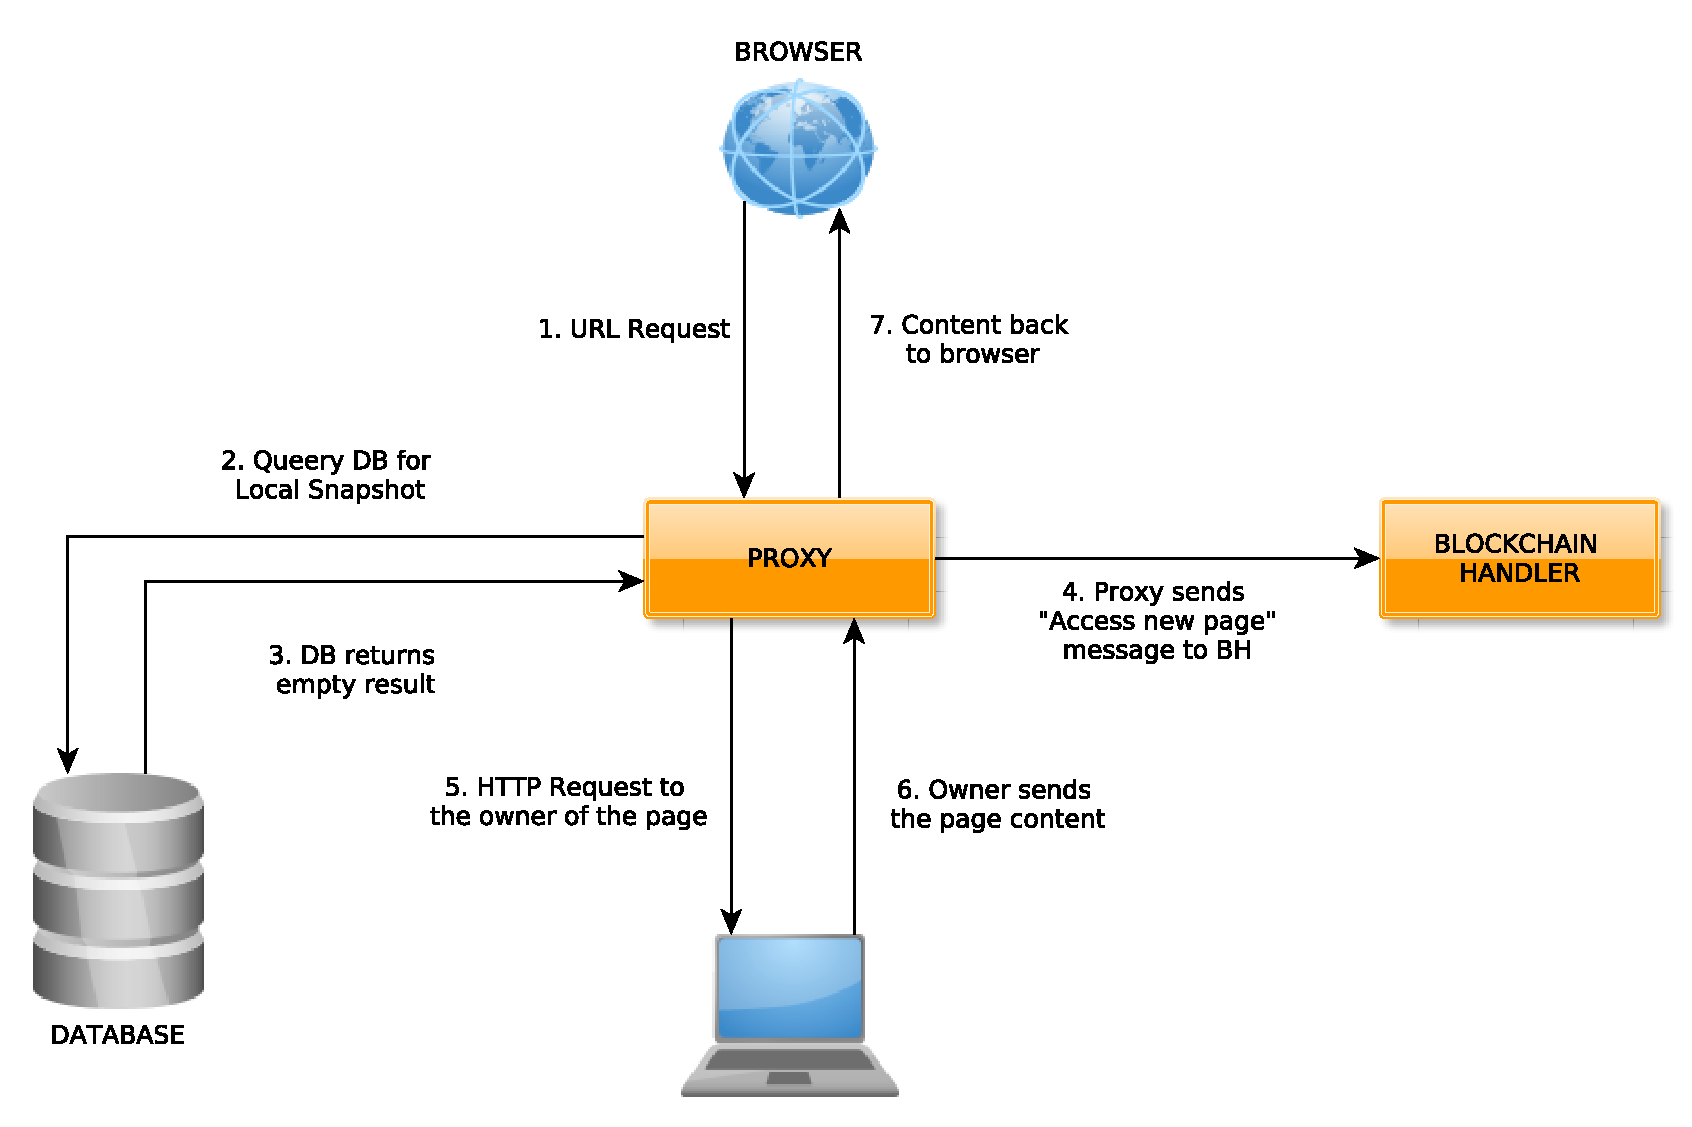
\includegraphics[width=0.5\textwidth]{pictures/fetch_page_online_creator.pdf}
\caption{First access of a web page whose creator is online.}
\label{fig:online_creator}
\end{figure}

In particular, when the user types the \texttt{url} of his choice in his browser the proxy is
triggered and makes a query to the local database. The local database returns an empty result,
which is interpreted as absence of a stored snapshot and the blockchain for this page.
Accordingly, the proxy sends a message to the Blockchain Handler that is going to access 
a web page for the first time and makes an HTTP request to the owner of the web page. 
The message to the Blockchain Handler is essential because this is the component that stores 
statistics and decides which pages are hosted. Finally, the owner responds to the HTTP request
and the user accesses the page.

\subsection{Page request for a page who's owner is offline}

\begin{figure}[htp]
\center
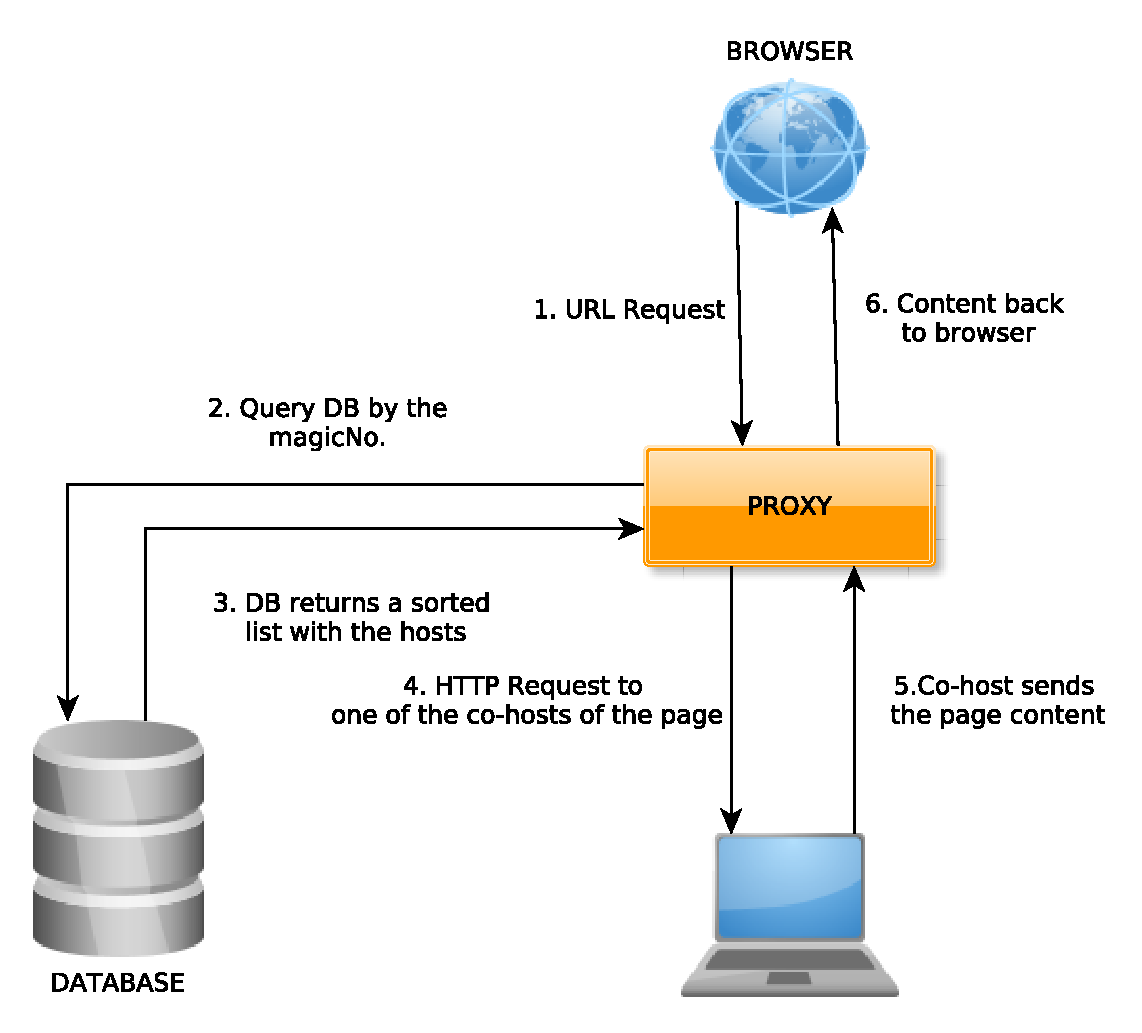
\includegraphics[width=0.4\textwidth]{pictures/fetch_page_offline_creator.pdf}
\caption{A node fetches a page from a co-host because its creator is offline.The 
blockchain of the page is stored locally.}
\label{fig:offline_creator}
\end{figure}
